%!TEX root = ../main.tex
%TODO: Redo the flowchart with updated and more specific steps

The input to our problem is a fiducial marker $F$ that provides the object position in the real world, and a 3D mesh $M$ that will be rendered in Augmented Reality. The method will calculate the properties of a set of light sources $L_i$, specifically position, rotation, intensity and color. In order to analyze the luminance ($L()$), a $360^{\circ}$ panoramic image is required, generated as a pre-processing step as explained in chapter \ref{theory}. The complete process is depicted in the flowchart in Figure \ref{flowch}, and each step is consequently described in more detail according to the mentioned sections.
\begin{figure}[H] 
  \centering
  \setlength{\unitlength}{\textwidth} 
    \begin{picture}(1,0.5)
       \put(-0.1,0){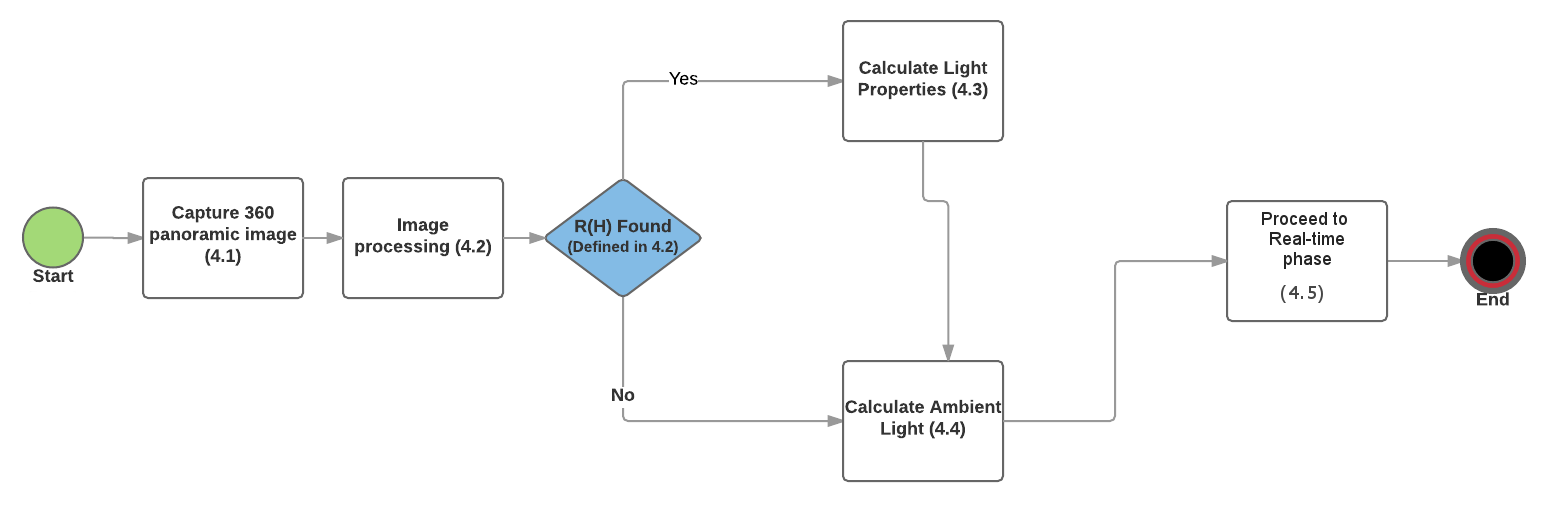
\includegraphics[width=1.3\unitlength]{Figures/Flowchart.png}}
       
    \end{picture}
    \caption{Our method in a nutshell.}
    \label{flowch}
\end{figure} 

\section{Capture $360^{\circ}$ panoramic image}
We use panoramic images as a pre-process. As such it's not within the scope of the method to define a new way of capturing $360^{\circ}$ images. The application we used to procure a spherical panoramic image within the device itself is Google Street View. This application guides the user through the process of generating the $360^{\circ}$ panorama. In total 44 photos are necessary and the application shows an orange dot on the screen on the point where the user has to point the camera next. This functionality was originally conceived to capture outdoors scenes, but if the user stands roughly in the middle of a room it works to capture indoors scenes as well.\newline
We ask the user to provide the origin of the virtual world by rotating the virtual reflective sphere so that the view of the room aligns with that of the section of the real room that the camera is facing. This also simplifies calculations of light orientations later on.

\section{Light source filtering}\label{lsf}
We factor out the luminance from the RGB representation of the panorama. This is achieved by the following equation:
\begin{equation}
  \forall \  P_{ij}; L(P_{ij}) = 0,2126 \cdot R_{ij} + 0,7152 \cdot G_{ij} + 0,0722 \cdot B_{ij} ,
\end{equation}
where $L$ is the luminance obtained at D65 white point and $P$ is the pixel in the $i,j$ position of the image and $R,G,B$ are the red, green and blue components of the pixel, respectively. \newline
The contrast ratio has to be adjusted, so that the regions with high luminance are more clearly separated.

\begin{equation}
     g(i,j) = \alpha \cdot L(P_{ij}) + \beta
\end{equation}

Where $g(i,j)$ is the adjusted image, $L(i,j)$ is the original grayscale image and $\alpha$ and $\beta$ are the brightness and contrast constants respectively, determined by parameter tuning. We carried out the parameter tuning in a trial-and-error basis, by using initial extreme values and run the program, and varying the values in order to achieve the best result. The values that worked in the implementation were $\alpha = 220$ and $\beta = 255$.
In order to prevent outlier pixels and noise from causing false positives, we normalize $g(i,j)$ as follows:
\begin{equation}
    N(g_{ij}) = \frac{ 2 \cdot g_{ij} }{min(L) + max(L)},
\end{equation}
Where $min(L)$ and $max(L)$ are the overall minimum and maximum luminance values in the image. 
\newline
The result of these steps is a black and white image with the rough shape of the light source. We call these shapes \emph{regions of high luminance}. If there are no regions of high luminance in the image at all it means that no relevant light sources were found. A region of high luminance in the image is formally defined as follows:
\begin{equation}
    R(H) = \{p_{00}, p_{01}, ... , p_{mn}\},
\end{equation}
 where $p_{ij}$ is the pixel in the i,j position of the image, so that 
\[
    L(p_{ij}) \leq 0.9 \cdot max(L(p_{ij})) 
\]
The region must also be connected side-by-side, so the pixels must be adjacent.\newline
Regions of high luminance are for the most part characterized by much noise and artifacts. These are caused by clear objects, reflections of light sources on polished surfaces, and even light sources that are far away, but don't contribute an important amount of light to the area of interest. Therefore, it's necessary to also add further filtering to the pipeline. \newline
The amount of light that a lighting source contributes to a given scene is directly proportional to the emission area of that source. When analyzing a photograph this area translates to the pixel size of the light source in the image. So we consider this to be a good measure for filtering. Figuring what constitutes an acceptable region size to determine if we have to filter a the light source is a challenging problem for which we couldn't find an existing solution. The approach we took is to define a percentage of the width and height of the overall image as a threshold in search for the best solution. The size filter is then:
\begin{equation}
    width(R(H)) \cdot height(R(H)) \geq k \cdot W \cdot H
\end{equation}
Where $k$ is the threshold, in the implementation the value that yielded the best results was $k = 0.004$; $W$ and $H$ are the total image width and height.\newline
Each identified region of high luminance that passes all the filters is a light source used at runtime. We capped the maximum amount of light to 8 in practice. We decided to use a maximum of 8 for a few reasons. With more than 8 light sources it becomes challenging to keep the scene from being too lit, even normalizing the intensities. Since we're calculating shadows for each light source, we found that doing it for more than 8 light sources made this process a bottleneck that caused the whole application performance to drop. \newline

\section{Calculate light properties}
We need to calculate position, orientation, intensity, and color for each light, remembering that we have the original full color image available.  \newline
\begin{enumerate}
\item  \textbf{Orientation}: This process is carried out with an array $P_i$ of points containing the pixel coordinates $(x,y)$ of the regions of high luminance; the normalized luminance analysis image $N(g_{ij})$ mapped on a sphere $S$ and a camera $C$ facing the sphere from four different points of view (in order to cover a full revolution). The orientation of the pth light source $O(L_p)$ is calculated as follows:
\begin{algorithm}[H]
\caption{Light source orientation calculation}\label{alg:orientAl}
\begin{algorithmic}[1]
\For{\texttt{i $\in[1,4]$}}
    \For{\texttt{each pixel in camera view}}
        \State \texttt{Cast ray to $S$}
        \If {Color at hit point $H$ is white AND $H=P_p$}
            \State \texttt{Calculate $O(L_p)$:}
            \begin{equation}
            O(L_p) = -2 \cdot (N_h \cdot C_r) N_h + C_r,
            \end{equation}
            \NoNumber{ $N_h$: normal of $S$ at $H$.}
            \NoNumber{$C_r$: camera ray direction.}

            \State \texttt{Normalize $O(L_p)$:}
            \begin{equation}
            O(L_p)_N = (\frac{O(L_P)_x}{|O(L_P)|}, \frac{O(L_P)_y}{|O(L_P)|}, \frac{O(L_P)_z}{|O(L_P)|})
            \end{equation}
        \EndIf
    \EndFor
    \State \texttt{Obtain the next camera view by rotating $C$ $90^{\circ}$ clockwise around the $y$ axis of $S$}
\EndFor
\end{algorithmic}
\end{algorithm}
This process is depicted in Figure \ref{camMov} for further clarification. The figure shows the vectors $N_h$ and $C_r$, the $C$ orbiting $S$ and the four distinct points of view with which $C$ reconstructs the entire $360^{\circ}$ environment.
\begin{figure}[H] 
  \centering
  \setlength{\unitlength}{\textwidth} 
    \begin{picture}(0.75,0.5)
       \put(-0.1,0){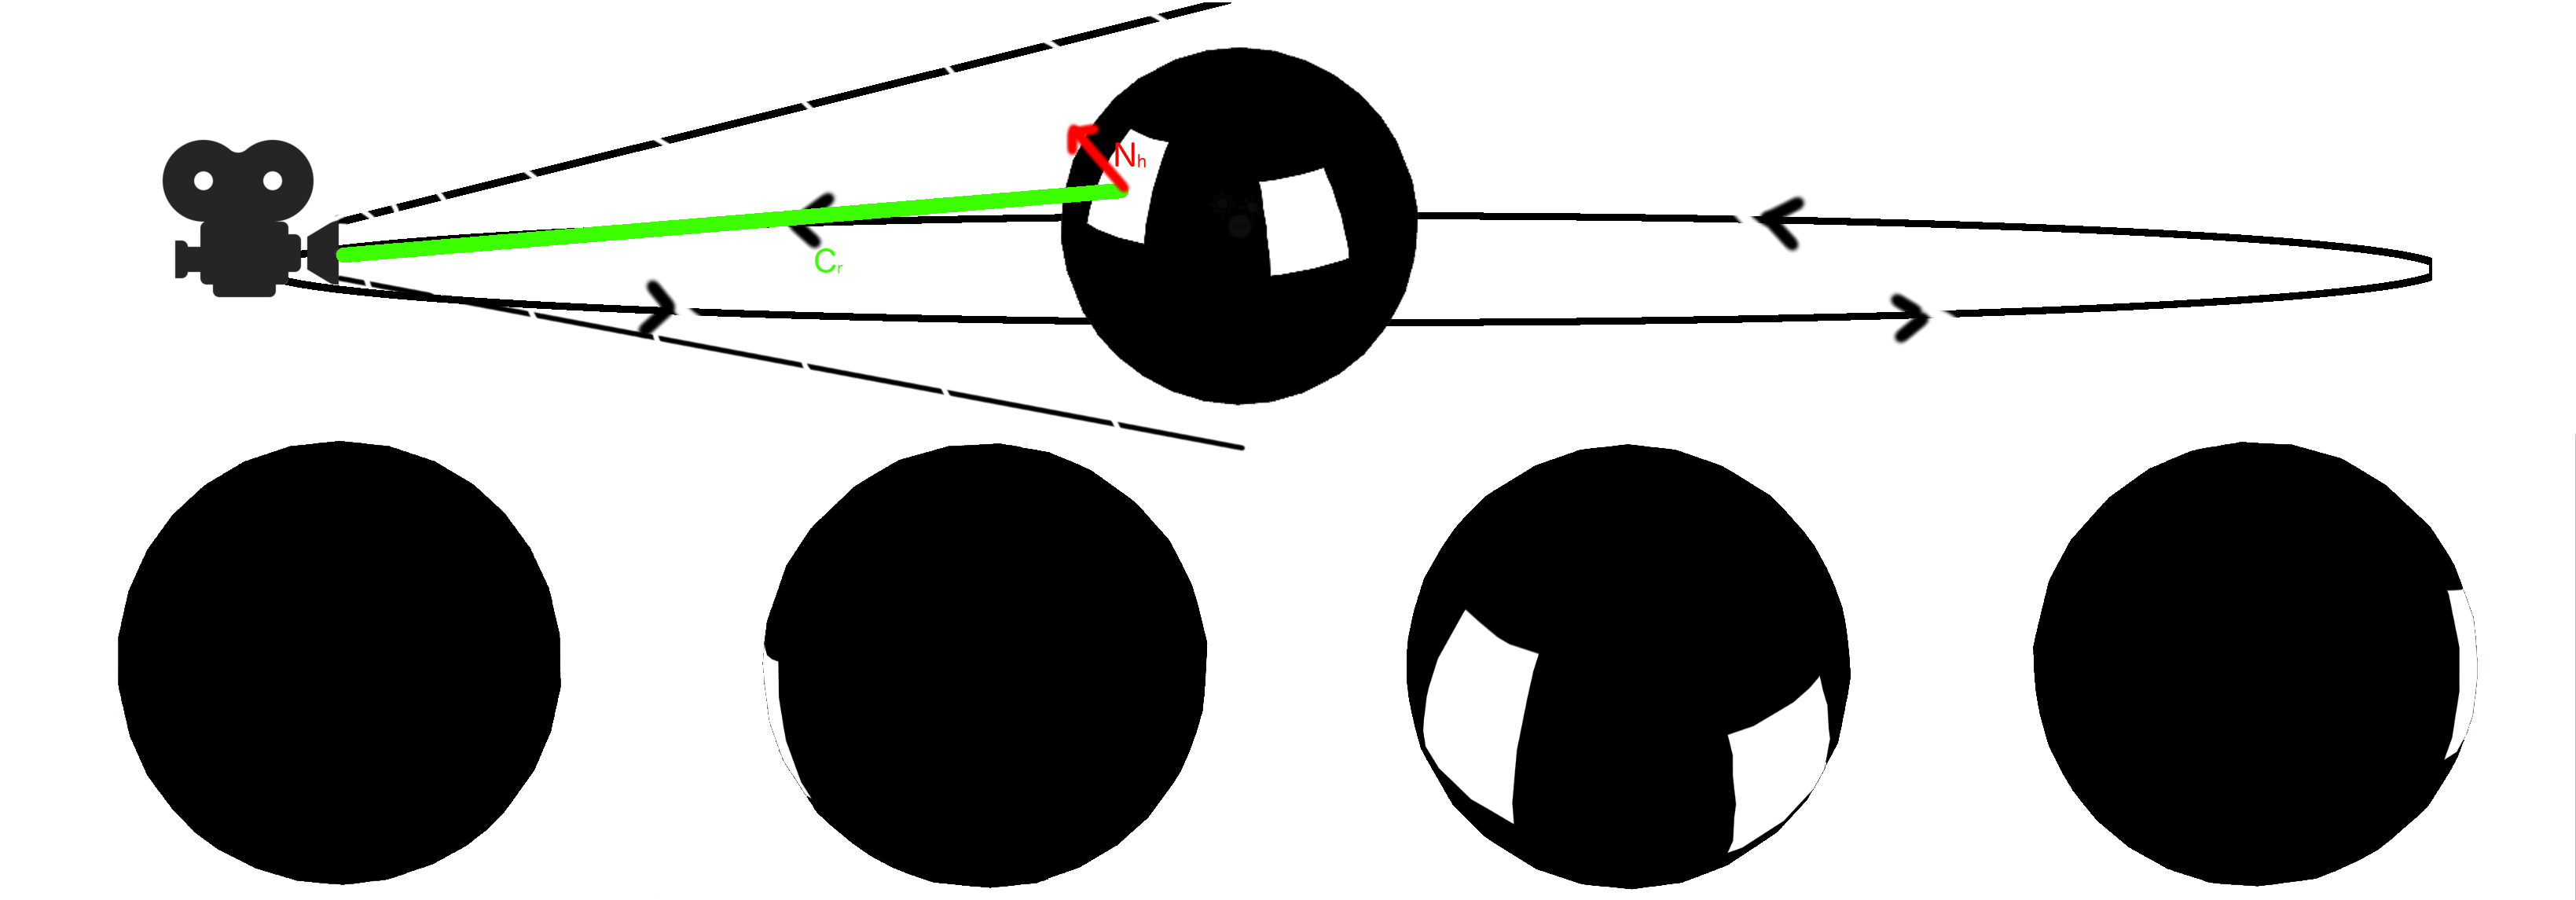
\includegraphics[width=1.0\unitlength]{Figures/camMov.png}}
       
    \end{picture}
    \caption{Illustration of the computation of the light orientations based on the virtual reflective sphere.}
    \label{camMov}
\end{figure} 
\item \textbf{Position}: With the orientation calculated in the previous step we know the angles of the light source with respect to the marker $F$. What we don't know is how far away along that vector the light actually is. In order to approximate the distance from a camera to an object in a photograph we can use triangle similarity, the device's known camera parameters and a known object size. The ratio of the size of the object on the camera sensor and the size of the object in real life is the same as the ratio between the focal length of the lens and distance to the object.
We use the average of a light source's height to approximate the desired distance:
\begin{equation}
   D = \frac{f \cdot h(O_r) \cdot h(L)}{h(O_p) \cdot h(s)},
\end{equation}
where $f$ is the camera aperture size, $h(O_r)$ and $h(O_p)$ are the real object height in millimeters (the value we used is 200 mm) and the image object height in pixels, respectively; $h(L)$ is the height of the full image and $h(s)$ is the camera sensor height.

\item \textbf{Color}: Storing both versions of the panorama, one in full color and another one after processing, allows us to have both the color and the luminance information. Once a light source is detected, the equivalent area in the color image is averaged to determine the color of the light source. We obtain the linear average of each individual color channel and use the combined results.
\item \textbf{Intensity}: There are two factors that influence the intensity of a light as perceived by a camera, the light size and the color temperature. The light's color temperature in Kelvin is calculated using the approximation proposed by \citep{mccamy1992}, as follows:
\begin{equation}
    T(C_p) = -949.86315 + 6253.80338 ^ {\frac{-n}{0.92159} } + 28.70599 ^{\frac{-n}{0.20039} } + 0.00004 ^ {\frac{-n}{0.07125} }
\end{equation}
\begin{equation}
n = {\frac{0.23881\cdot R + 0.25449\cdot G - 0.58291\cdot B}{0.11109\cdot R - 0.85406\cdot G + 0.52289\cdot B} }
\end{equation}

Where $R, G, B$ are the red, green and blue components of the light color.\newline 
The other significant factor to determine the light intensity is the size. In our method the size is given by the integral of the region of high luminance with respect to the full image.\newline
The light intensity is finally expressed by:
\begin{equation}
I(L_p) = T(C_p) \cdot \int_{R(L_p)} N(g_{ij}) \,d\mu
\end{equation}
Where $N(g_{ij})$ is the output image of the luminance analysis and $R(L_p)$ is the $p^{th}$ region of high luminance. $I(L_p)$ is the scalar value that denotes the intensity of the light source at runtime.\newline 

\end{enumerate}

\section{Calculate ambient light}
Since a panoramic image of the environment is already available, we can use it to implement environment mapping. However, asking the user to capture the environment more than once in order to carry out the Tone Mapping would have a bad impact on user friendliness. It is also highly unlikely that the produced image would have the exact same framing every time. Alternatively, we produce the different exposure values for the Tone Mapping by altering the brightness and contrast values of the base image using equation 4.2 once again. Afterwards, we produce the HDR image using the \citet{Debevec} weighting algorithm.\newline

\section{Real-time Phase}
We use the original spherical panoramic image to create a cubemap of the real environment for ambient lighting, to calculate the ambient contribution of the diffuse shaders and to use as reflections for the specular shaders.
\begin{enumerate}

\item \textbf{Cubemap:} We take the polar coordinates of a unit sphere $(1,\theta,\phi)$. The image coordinates are divided into four regions by latitude $-\pi/4 < \theta < \pi/4 , \pi/4 < \theta < 3\pi/4, 3\pi/4 < \theta < 5\pi/4, 5\pi/4 < \theta < 7\pi/4$. These represent either one of the four faces of the cube, top or bottom. The projected coordinates are given by:
\begin{equation}
P_c = (1, tan(\phi), \frac{cot(\theta)}{cos(\phi)}),
\end{equation}
 The process is further explained in Figure \ref{cubeMap}.
 \begin{figure}
  \centering
  \setlength{\unitlength}{\textwidth} 
    \begin{picture}(0.75,0.5)
       \put(-0.1,0){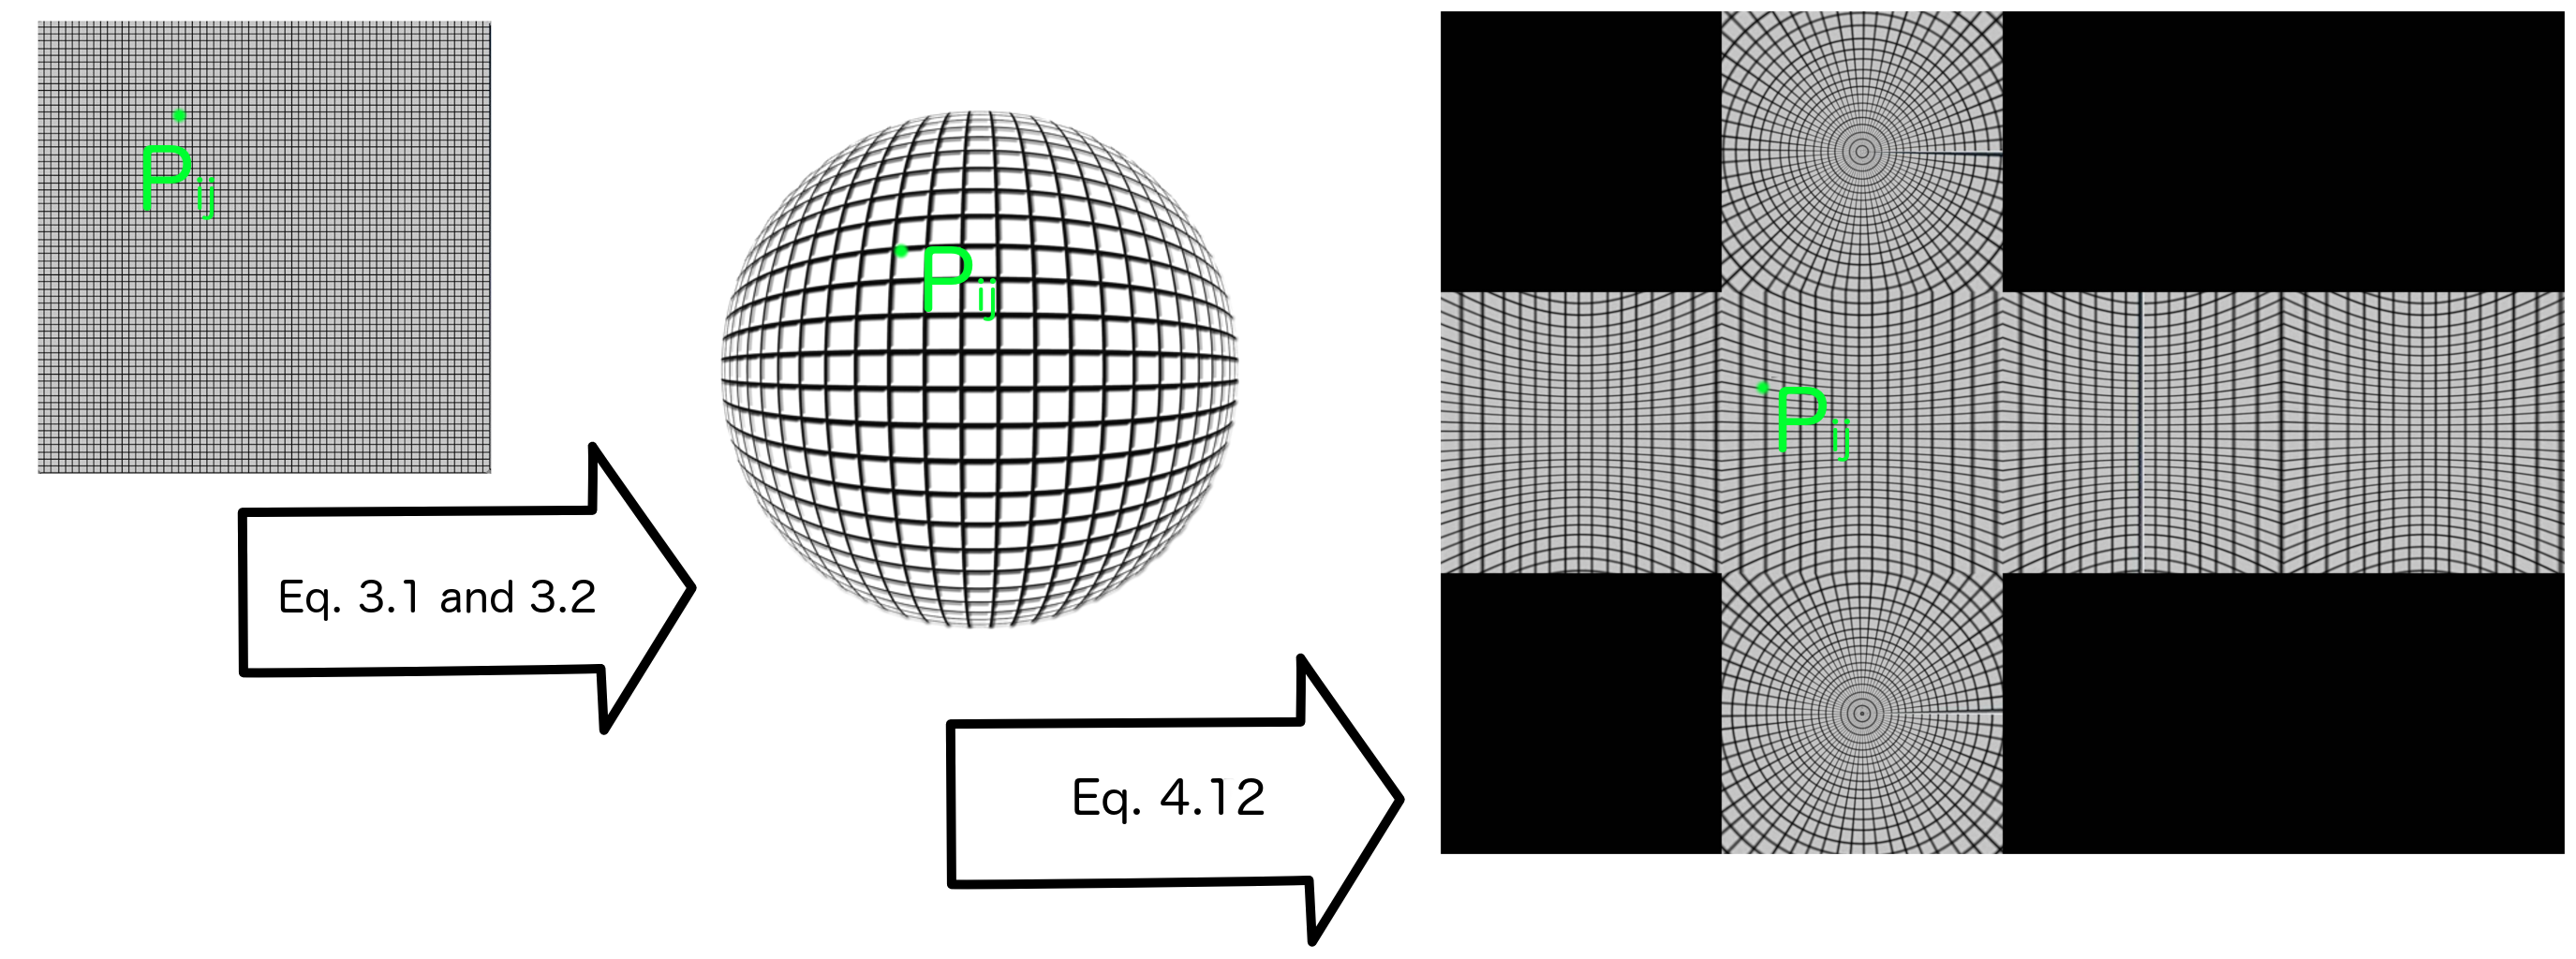
\includegraphics[width=1.0\unitlength]{Figures/cubemapping.png}}
       
    \end{picture}
    \caption{The cubemap creation process.}
    \label{cubeMap}
\end{figure} 
 
 The projected points for each face of the cube are composed into an image and each image stitched together to create a cross cube map.
 
 \item \textbf{Ambient contribution:} The environment lighting contribution is done with a shader. The ambient contribution is reduced to a single value in the range of $0$ and $1$ and applied to the diffuse color component. The result is a dimmer color when the ambient light is low. 
 The ambient contribution value $A_c$ for each region of high luminance $R(L(P_{ij}))$ in the luminance analisys image $N(g_{ij})$ is given by:
 \begin{equation}
 \forall R(L(P_{ij}));A_c = \frac {\sum_{i=1,j=i} R(L(P_{ij}))}{width(R(L(P_{ij}))) \cdot height(R(L(P_{ij})))}
 \end{equation}
 
 \item \textbf{Reflections:} The cubemap from step 1 is also used to for reflections. A vector is cast from every vertex of the object along its normal and intersected with the cubemap generated from the panoramic image. The texture color is mixed with the diffuse color according to the specularity defined for the material to simulate reflection, this information is calculated in advance and used at runtime. 
 
 \item \textbf{Shadows:} During early experiments it became clear that one of the bigger differences between real and virtual object were a product of the shadows as well as the light. A problem when it comes to casting shadows for virtual objects in AR is the fact that there has to be an object underneath $M$ to cast the shadow on. But this object has to be as unobtrusive as possible. We worked around this issue by using a transparent material on a plane that receives shadows. $M$ is projected on the plane from each light source and rendered flat in black color.
 
\end{enumerate}